\documentclass[12pt, oneside]{book} 
\pagestyle{plain}

% The \usepackage{} command will import predefined fonts, symbols, environments, etc.  For example, the ams packages below come from the American Mathematical Society and include all kinds of useful math symbols like integrals
\usepackage{amscd}
\usepackage{amsmath}
\usepackage{amssymb}
\usepackage{amsthm}
\usepackage{verbatim}
\usepackage[utf8]{inputenc}
\usepackage{geometry}                		% See geometry.pdf to learn the layout options. There are lots.
\geometry{letterpaper}                   		% ... or a4paper or a5paper or ... 
%\geometry{landscape}                		% Activate for for rotated page geometry
\usepackage[pdftex]{graphicx}				% Use pdf, png, jpg, or eps with pdflatex; use eps in DVI mode	
\usepackage{setspace}
\usepackage{physics}
\usepackage{subcaption}
\usepackage[numbers]{natbib}
\usepackage{pdfpages}
\usepackage{pgfplots}
\usepackage{bm}
\usepackage{wrapfig}				% enables the use of \wrapfig, for figures with text wrapped around them
\usepackage{afterpage}
\newcommand\blankpage{%
    \null
    \thispagestyle{empty}%
    \addtocounter{page}{-1}%
    \newpage}

\usepackage{bibentry} % for list of publications
\usepackage{hyperref}

% \usepackage[english]{babel}
\graphicspath{{images/}{{\subfix{images/}}}}
\usepackage{tikz}
\usepackage{tikz-3dplot}
\usetikzlibrary{shapes,calc,positioning}
\tdplotsetmaincoords{70}{120}
\usepackage{siunitx}
\usepackage{adjustbox}
\usepackage{xcolor} %% Text color
\usepackage{blindtext}
\usepackage{subfiles} % Best loaded last in the preamble
\usepackage{multicol,multirow}  %% Figure in two columns
\usepackage{mathtools, nccmath}

\usepackage{lipsum}			% gives access to \lipsum, which dumps some latin text into your document as filler if you want to check formatting

%\usepackage[parfill]{parskip}    		% Activate to begin paragraphs with an empty line rather than an indent



% Here we set the page dimensions to match the standard thesis format.  These values should not be changed.
%%% SET LENTGH AND WIDTH %%%
\setlength{\textwidth}{6.5in}
\setlength{\textheight}{8.5in}
\setlength{\oddsidemargin}{0pt}
\setlength{\evensidemargin}{0pt}
\setlength{\topmargin}{0pt}
\setlength{\marginparsep}{0pt}
\setlength{\marginparwidth}{1in}


%\begin{document} starts LaTeX looking for actual content.  Everything above this point is purely formatting.
\begin{document}

\begin{titlepage}
\begin{center}

% \vspace* creates some vertical white space on the page to make the title page look more pleasing.  \vspace would do much the same thing, but would not insert the white space if we were at the top of a fresh page.  As this is the start of the document we're obviously at the beginning of a page, so the asterisk is necessary to ensure we still put in two cm of white space.
\vspace*{2cm}

{\Large \textbf{Parallel Search: A* with CUDA}} % \huge sets the font size.  Other options include things like \large, \Large, \small, \tiny, etc.

\vspace{5cm}
{15-418 Final Report}

\vspace{2cm}
{\large \textbf{Aditya Kannan}\\ \textbf{Gabriel Lee}}
% \vfill creates an arbitrary amount of vertical white space as necessary to fill the page
\vfill

May 2022

% \vspace*{3cm}

\end{center}
\end{titlepage}

% \frontmatter defines the pieces of the thesis which will use roman numerals for page numbering


% \chapter{} and/or \chapter*{} will create a chapter in your thesis.  Including the asterisk will cause the chapter to not appear in the table of contents.


\chapter{Summary}

We developed an approach to implement the A* algorithm in parallel called GA*. A* is a classical search algorithm that is used for computing the optimal path between a source and a sink node. We develop several data structures, optimized for use in parallel applications, and designed an algorithm that allows us to run A* efficiently on a GPU. We implemented a serial version of A* and sequential version of the GA* algorithm. While we made many attempts at creating GA* in CUDA, we were ultimately unsuccessful in this endeavor. We applied the A* problem to a slider game. We demonstrate the solution generated by our algorithm in a visual demonstration of the solution to the sliding game.



\chapter{Background}

\section{The A* Algorithm}

The A* algorithm is a solution to the single source shortest path problem. It is applied on a graph (directed or undirected) with various costs for all the edges of the graph. A* finds the path of edges from a given source and goal node that minimizes the total sum of the edge costs.
\newline\newline
It improves on algorithms like Dijkstra's algorithm by using a heuristic to help guide the search for the end goal. Every node $n$ in the set of vertices $V$ has a distance $g(n)$ from the source node that was discovered by exploring the different paths from the start to $n$. There is also a heuristic function $h$ such that $h(n)$ represents an estimate of the remaining distance to the goal node. Nodes on the frontier of the search are placed on a priority queue. They are then picked to be explored from the frontier based on a combination of the cost and heuristic functions: 
$$f(n) = g(n) + h(n)$$
By using $f(n)$ to prioritize nodes that we believe are more likely to reach the goal faster, we are able to expand fewer nodes and find the least cost path more efficiently then Dijkstra's algorithm.
\newline\newline
In order to ensure that we have an accurate estimate of the priority of a node, we need our heuristic to be consistent in order for the A* algorithm to generate a provably correct output. A heuristic is consistent if for a node $s$ and any of its neighbors $s'$, it satisfies the following inequality:
$$f(s) \le d(s, s') + f(s')$$
where $d(s, s')$ is the distance between the two nodes.

\begin{figure}
    \centering
    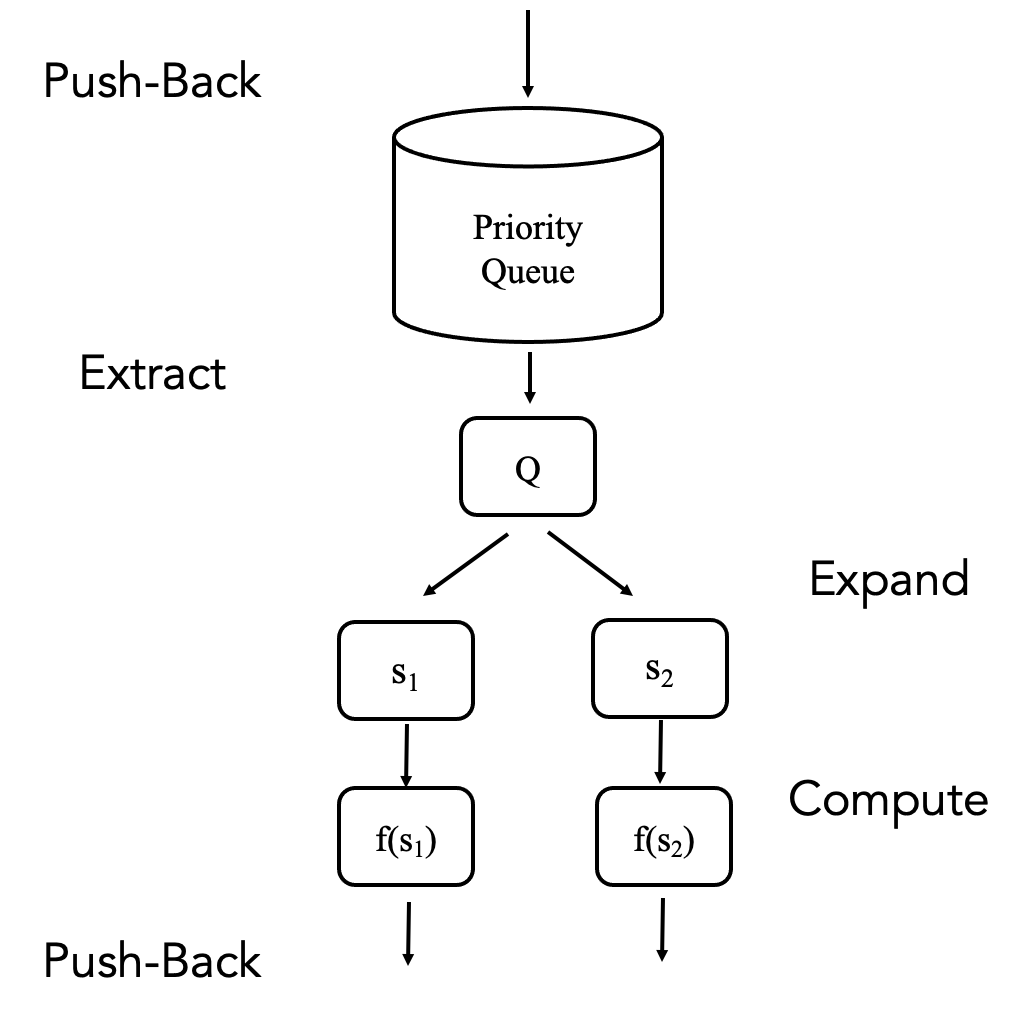
\includegraphics[scale=0.5]{figures/astar.png}
    \caption{A* workflow}
    \label{fig:astar}
\end{figure}

\section{Algorithm (GA*)\cite{paper}}

The A* algorithm as described above is \textbf{not amenable to parallelization}. The priority queue requires that only the topmost entry in the priority queue be used for exploration. As a result, it is not possible to create a parallel version of the algorithm described above without changing the data structures.\newline\newline
GA* is a general version of A* that can be run in a parallel setting. We present the pseudocode of our algorithm below:

\begin{verbatim}
let GA start target =
    let Q = {q1, q2, ..., qk}       // set of priority queues (open list)
    let H = {}                      // global hash table (close list)
    let m = None                    // state pointer (found goal)
    
    q1.push(start)
    while not all q in Q empty do
        let S = []                  // global list (expanded states)
        
        parallel for i in [0, k] do
            if qi empty then break
            
            // every thread expands one state
            let si = qi.pop()
            
            // update goal state if found state is shorter path to goal
            if si = t then
                if m = None or si.total_cost < m.total_cost then
                    m <- si
                break
            
            // add neighbors
            S.extend(s' for s' in s.next)
        done
        
        // check if found goal state is closer than all other states
        if m != None and m.total_cost <= min si.total_cost then return m.path
        
        // remove expanded states that have already been seen cheaper
        parallel for i in [0, s.length] do
            if si in H and H[si] < si.path_cost then s.pop(i)
        done
        
        parallel for i in [0, s.length] do
            // push si to some q in Q evenly
            Q.push(si)
            
            // store seen expanded paths
            H[si] <- si.path_cost
        done
    done
    return m

\end{verbatim}
At a high level, this algorithm uses \textbf{multiple priority queues} to generate a path between the start state and goal state. An explicit graph data structure is unnecessary in this scenario as we can determine neighbor states from the current state (and anyways, an explicit graph structure would be very much too large in scenarios that would motivate parallelization on this scale).\newline\newline
The pseudocode is commented at each step, but the high level idea is that each thread has its own priority queue of states. Each thread expands the top node of its own priority queue, checks if it has reached a goal state and if it has been visited already and expands the neighbors of this state.\newline\newline
When states are expanded, the number of states grows exponentially, resulting in a smoothing of the states distribution across all of the threads. This results in \textbf{state duplication} among independent threads that may separately want to push the same state onto the frontier. To handle this, we need to keep track of which nodes have been explored and/or will be on the frontier. We utilize the global hash table (described below) for this purpose.

\section{Data Structures}

\begin{figure}
    \centering
    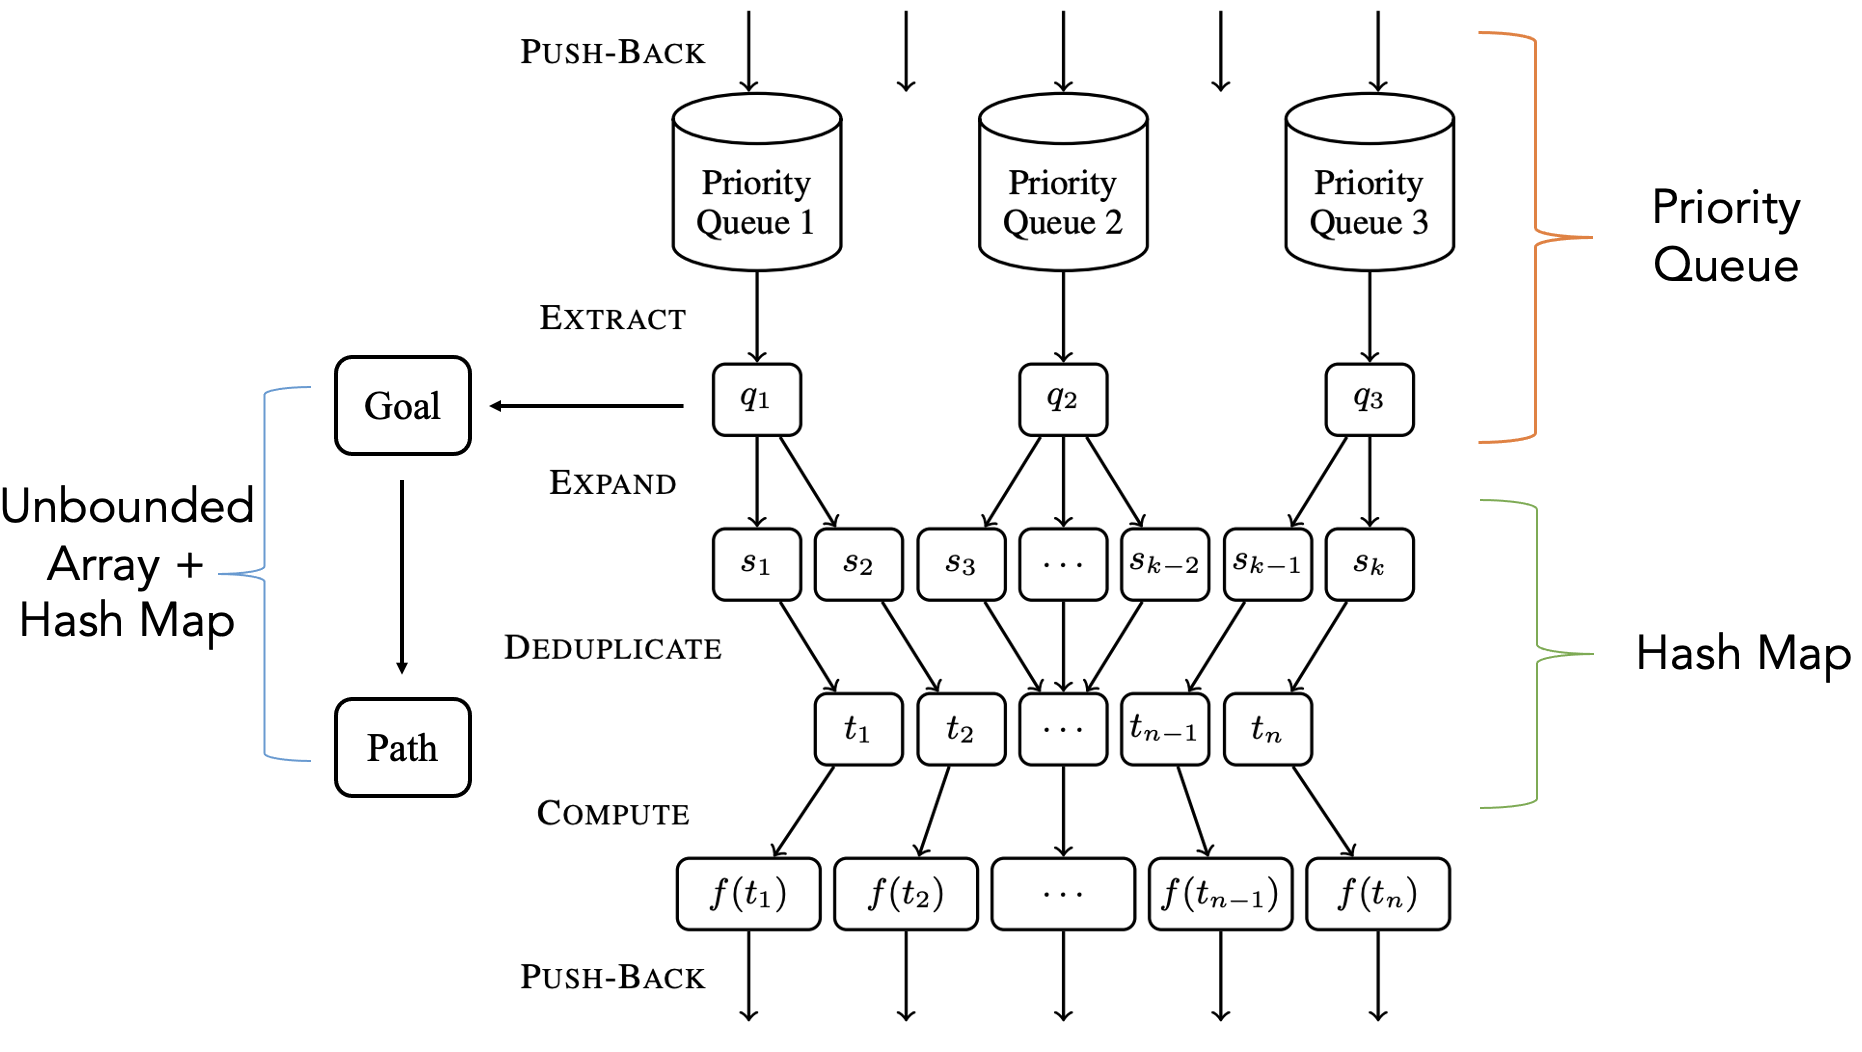
\includegraphics[scale=0.5]{figures/gastar_ds.png}
    \caption{GA* workflow with relevant data structures (based on \cite{paper})}
    \label{fig:gastar_ds}
\end{figure}

\subsection{Serial}
Standard libraries cannot be used in CUDA code due to GPU memory working differently than CPU memory. Thus, certain serial data structures need to be re-implemented to accommodate for this.
\subsubsection{Unbounded Array}
This structure is used to generate the path to the goal state once the algorithm terminates. Thus, unlike a standard unbounded array, it only requires a \texttt{push} operation. It has a growth factor of $2$ (resize to double its original size).
\subsubsection{Priority Queue (Heap)}
Every thread contains their own priority queue for expanding states. These are min-heaps (for retrieving closest perceived state) that operate on top of an unbounded array structure (same as above, but with a shrinkage factor of $2$ as well). In accordance with the above algorithm, they have \texttt{pop}, \texttt{push}, and \texttt{is\_empty} operations.
\subsection{Parallel}
\subsubsection{Hash Table (Parallel Hashing with Replacement)\cite{paper}}
This structure is used to keep a global collection of visited states and their path costs. Because of this global attribute, this is the bottleneck in the algorithm. A standard hash table contains an unbounded array of linked lists, but the structure's dynamic nature (on item inserts) makes it extremely difficult to parallelize. To tackle this problem, we implement parallel hashing with replacement\cite{paper} which uses a static list and multiple hash functions. The second hash function can search for new locations in the table for a node if another element collides with it in the first hash function. Our rationale for choosing this structure is explored in the Approach chapter. As in a standard hash table, this has assignment, existence, and modification operations. These operations are allowed to run in parallel with one another and must be thread-safe.

\section{Workload}
In the sequential algorithm for A*, a single priority queue is used to determine the next state to extract. Since node neighbors are fully dependent on the nodes within the priority queue, this data structure becomes the bottleneck if we were to parallelize the algorithm. If instead (as demonstrated in the pseudocode), we allow for states to be expanded independently of one another using multiple independent priority queues, we will allow for duplicate expansions. Thus, especially for large problem spaces, the approach is massively parallel.\newline\newline
Since each thread operates independently in the sense that they expand nodes without dependencies on nodes held by other threads, \textbf{this program is task parallel}. Locality and vector instructions are not as relevant due to this.

\chapter{Approach}

\section{Setup \& Hardware}
All of our code was written from scratch.\newline\newline
The goal of our project was to create a working GA* implementation on GPU. To this end, we used C++ for serial implementations and CUDA programming to develop our GPU code. We evaluated our code on the GHC machines.\newline\newline

\section{Work Distribution}
The parallelism of our work comes from how we explore the frontier of the A* search more efficiently. The original A* algorithm as designed for sequential execution is not amenable to parallel speedup, so we used the GA* algorithm instead to judge parallel execution. \newline\newline
Each of our threads corresponded to one priority queue. It was responsible for popping the top node in the priority queue, and evaluating it for if it is the goal state and for finding its neighbors. With this approach, we could have \textit{thousands} of priority queues, which is especially useful in problems where the number of states increases exponentially, such as the slider problem we describe in the Results. In the rest of our algorithm, we encounter a lot of communication and synchronization. \newline\newline
We allocate a global array \verb|S| for storing all the neighbors that are being added to the frontier due to the expansion of the priority queue nodes. This array is accessible to all the threads. Once each thread generates the neighbors it expands in the current iteration, it adds those neighbors to \verb|S|.\newline\newline
We also allocate the hash table as a global variable. Once the threads populate the array \verb|S|, each thread works on deduplicating nodes in the array \verb|S| (not necessarily the nodes it added to \verb|S|!). This is done by looking at the global hash map for the same node and replacing it if there's a node in \verb|S| that has lower cost. If not, we discard this node from \verb|S|. \newline\newline
Finally, we redistribute the remaining nodes evenly to the many different priority queues. We do this by rearranging the indices in \verb|S| that correspond to the thread.

\begin{figure}
    \centering
    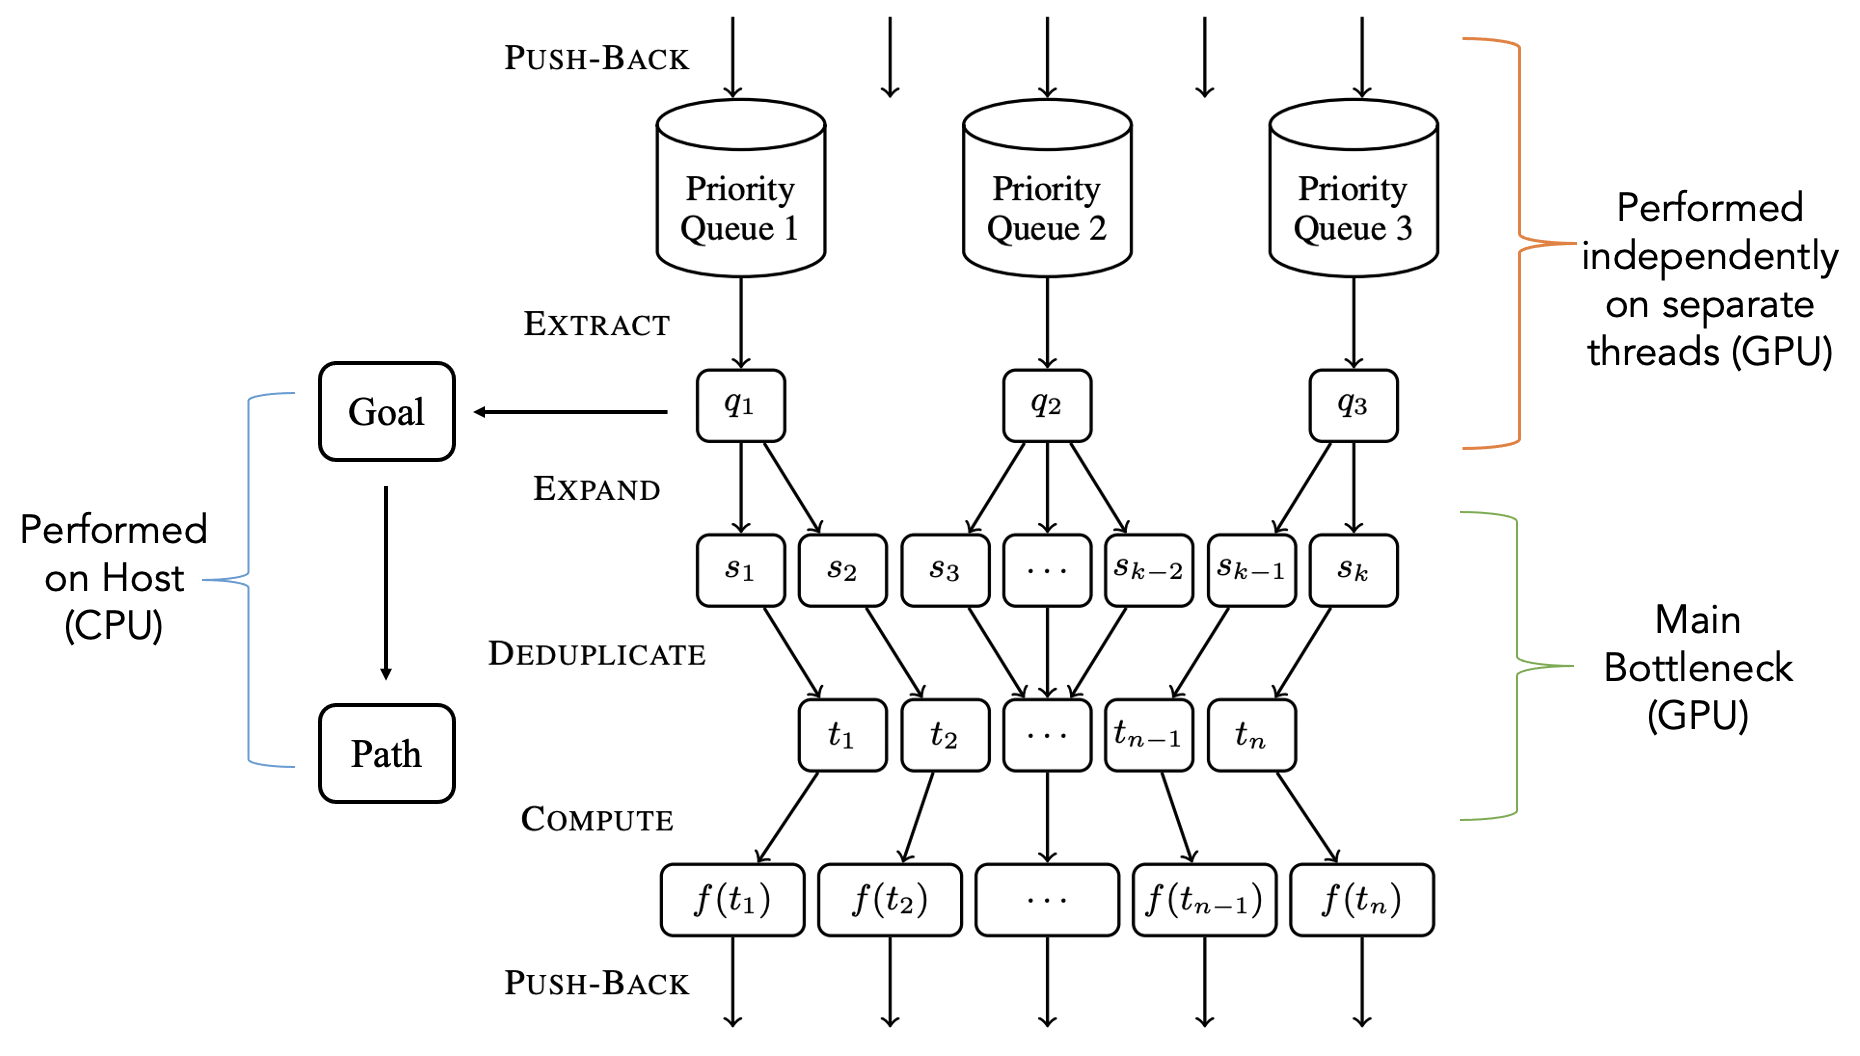
\includegraphics[scale=0.5]{figures/gastar_device.png}
    \caption{GA* workflow with relevant data structures (based on \cite{paper})}
    \label{fig:gastar_device}
\end{figure}

\section{Iterations of our Approach}
We began by implementing and verifying a sequential version of the original A* algorithm. These results are presented in the Results below. We then created a sequential version of the GA* algorithm that worked (i.e. it could run on a single CPU thread, not on CUDA. Nodes were mapped to a random priority queue so the structure imitated the final result we were hoping for). Finally, we made numerous attempts at a CUDA implementation for the GA* algorithm, but we were ultimately unsuccessful.\newline\newline
Along the way, we made a couple optimizations to our approach. We decided to allocate nodes in our frontier in \verb|S| in one ordering, and then \textbf{we redistribute the nodes to threads in a different order}. This way, by having nodes in different parts of the graph, the work done by the threads is evenly spread out. That is, we are less likely to run into situations where many priority queues are empty and do not have nodes to expand or add to \verb|S|.\newline\newline
Another idea we found was that we could optimize our deduplication to haves less synchronization and therefore potentially save time. There were two methods that \cite{paper} suggested for a parallel implementation of a hash table. The first one, Cuckoo Hashing, is a more complicated method that involved greater synchronization between threads. We opted to go with the second approach, Hashing with replacement, which required no synchronization at the cost of missing some duplicate nodes. We decided this tradeoff was acceptable because this approach would not affect the final path returned.

\chapter{Results}
\section{Sliding Game}
Our metric for algorithmic performance involves running A* on the sliding game (see the Youtube video for a demonstration). The sliding game is a particularly convenient search problem for two reasons: the state representation is small and the state space is very large. It blows up exponentially with respect to the puzzle dimensions. This is particularly important since our goal was to measure the effectiveness of a parallel A* algorithm, and the expansive state space would decrease potential overhead.
\newline\newline
\begin{tabular}{ |p{3cm}||p{3cm}|p{3cm}|p{3cm}|  }
\hline
\multicolumn{4}{|c|}{Sliding Game Sequential Execution times} \\
\hline
Board Size& Runtime (ns)&Runtime (ms)& Runtime (s)\\
\hline
2x3 & 35880 & 0 & 0\\
3x3 & 84711 & 0 & 0\\
3x4 & 258638033 & 259 & 0\\
4x4 & 171623957677 & 171624 & 172\\
\hline
\end{tabular}
\newline
\begin{figure}[h]
    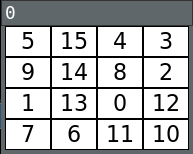
\includegraphics[scale=0.5]{figures/4x4.png}
    \caption{The puzzle grid used for the 4x4 measure}
    \label{fig:gastar_ds}
\end{figure}
\newline
The object of the game is to order the tiles in increasing numerical order. The 0 tile represents an empty tile where adjacent tiles can "slide" to. Thus, every turn can result in 4 more possible states (exponential). The graph below is a visual representation of the above runtimes in log scale.

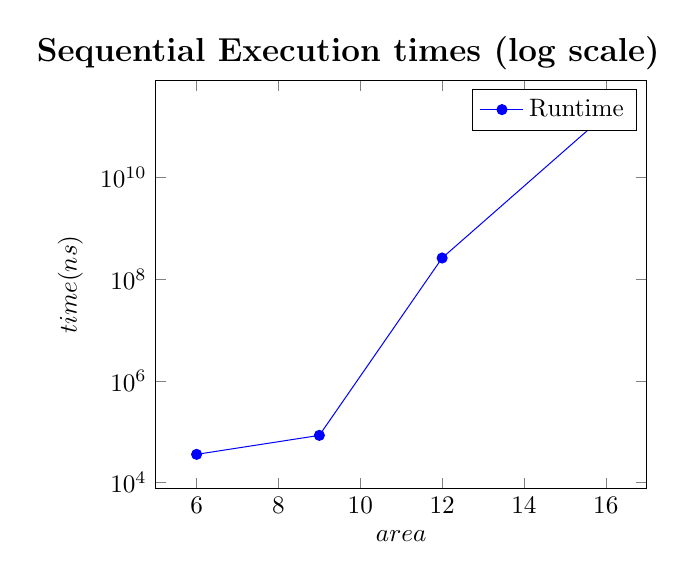
\begin{tikzpicture}[scale=0.91]
    \begin{axis}[
        xlabel=$area$,
        ylabel=$time(ns)$,
        ymode=log
                ]
    \addplot[mark=*,blue] plot coordinates {
        (6,35880)
        (9,84711)
        (12,258638033)
        (16,171623957677)
    };
    \addlegendentry{Runtime}
   
    \end{axis}
    \node[above,font=\large\bfseries] at (current bounding box.north) {Sequential Execution times (log scale)};
\end{tikzpicture}

\section{Evaluating Performance}
For this problem, we evaluated our implementations by checking the wall time of the implementations. We found this to be appropriate for the serial algorithm given that we were not able to properly evaluate speedup for the GA* GPU method.

\section{Scaling the Problem Space}
Considering our sequential performance in the graph above, we see that the line is roughly linear. This supports our hypothesis that as the number of cells grow, the runtime grows roughly exponentially. In particular, we see that because most nodes on the frontier have 3 or 4 neighbors, the number of states being added as we go further from the initial state increases exponentially. Due to the nature of the problem, a small change in workload could result in dramatically larger runtime.

\section{Limitations of our Approach}
The main source of issues with our CUDA implementation came from our hash map. Our implementation of the hash map involves a table and two hash functions where the second can search for new locations in the table for a node if another element collides with it per the first hash function. Although this simplification allows us to not need sychronization in this section, it means that we need a very large hash table. If the hash table is small compared to the number of states, it is possible that an element has collisions with both the hash functions. In this case, the hash map will \textit{lose information} that could potentially be important for the final path.\newline\newline
Another limitation of our approach was the amount of global memory that we allocate in this method. We use it for the large array \verb|S| as well as the hash table. If we scale up the hash table size in order to reduce the likelihood of collisions, we will increase the global memory allocated. In the GPU, global memory is far less efficient to update than shared memory. \textbf{As a result, the global memory brought upon by the hash table would likely be our main bottleneck in the CUDA implementation.}

\section{Changing the Hardware}
As we have discovered through this project, a GPU implementation of A* is not too pragmatic. In particular, the memory constraint of GPUs especially for search problems of this magnitude is quite restrictive. In contrast, using MPI would alleviate this. \textbf{MPI is not restricted by a single device and can be used across a network of devices, thus relaxing the space constraints}. Furthermore, MPI is a more task oriented system whereas CUDA is more data oriented, which is more suitable for search problems.

\chapter{Contributions}
There were two students in this project. The distribution was 50-50. The contributions are below:

\begin{itemize}
    \item \textbf{Gabriel Lee}: Serial A* implementation, Visualization code, IO code, GA* CUDA code, Written report contributions.
    \item \textbf{Aditya Kannan}: GA* sequential implementation, GA* CUDA code, Written Report, Presentation slides and video.
\end{itemize}

% the \appendix tag tells LaTeX where it should start labelling chapters with letters (denoting appendices) rather than numbers (denoting main chapters)
% \appendix 


% \bibliographystyle command to choose the format of your bibliography. More examples of bibliography styles can be found at https://www.overleaf.com/learn/latex/Bibtex_bibliography_styles
\bibliographystyle{unsrtnat}

% \bibliography is the command for the actual file containing your bibliographic data. This file can be produced manually or automatically using software such as BibTeX. Both options can work, however, learning to use BibTex is beneficial in the long run. An example of the format needed to generate your own bibliography file can be found as the bibliography.bib file here provided.

\bibliography{bibliography}

\end{document}